\chapter{Collaboratively generating ideas}
\noindent \textit{Learners worldwide collectively spend millions of hours per week testing their skills on assignments with known answers. Might some of this time fruitfully be spent posing and exploring novel questions? This chapter investigates an approach for learners to contribute scientific ideas. The Gut Instinct system embodies this approach, hosting online learning materials and invites learners to collaboratively brainstorm potential influences on people’s microbiome. A between-subjects experiment compared the performance of participants who engaged in just learning, just contributing, or a combination. Participants in the learning condition scored highest on a summative test. Participants in both the contribution and combined conditions generated novel, useful questions; there was not a significant difference between the two. Though participants in the combined condition both learned and contributed, this setting did not exhibit an additive benefit, such as better learning in the combined condition. These results highlight the promise and difficulty of double-bottom-line learning experiences}

%\begin{figure}[h] 
%  \centering
%  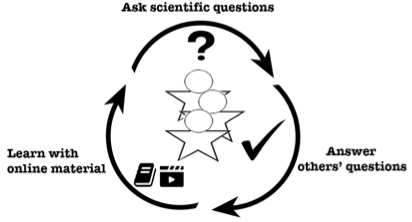
\includegraphics[width=1.0\textwidth]{figures/gutinstinct/gi-1.png}
%  \caption[]
%{A dual objective: integrating citizen science and online learning\index{gi-1}}
%  \label{fig:gi-1}
%\end{figure}

%%%%%%%%%%%%%%%%%%%%%%%%%%%%%%%%%%%%%
\section{The Promise of Citizen Science with Learners}

\begin{wrapfigure}{r}{0.5\textwidth}
  \centering
  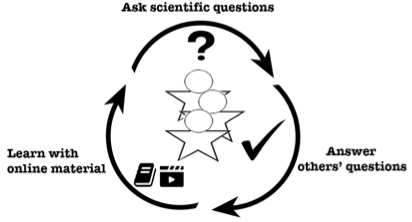
\includegraphics[width=0.5\textwidth]{figures/gutinstinct/gi-1.png}
  \caption[A dual objective: integrating citizen science and online learning]
{A dual objective: integrating citizen science and online learning\index{gi-1}}
  \label{fig:gi-1}
\end{wrapfigure}

People worldwide have theories about their health, environment, interpersonal interactions, and myriad other topics~\cite{Gelman2011}. Some of these folk theories encapsulate generalizable insights and wisdom; many others are completely false; and some are in between~\cite{Kempton1986}. How might we harvest and assess such intuitive theories to extend human knowledge, especially in domains where science is limited?  Worldwide, students collectively spend millions of hours a week testing their skills on assignments with known answers~\cite{Shah2015}. This community could be a potentially powerful resource. Repurposing even a small fraction of this effort towards scientific inquiry could pay significant dividends. 

Our intuition is that scientific crowdsourcing will most usefully contribute to domains where science is nascent and/or highly contextual. Knowledge of the human microbiome is both. While everyone has a gut full of microbes, its causal influences remain largely unknown. The Human Microbiome Project and other studies have begun revealing its diversity and impacts~\cite{Consortium2012, Consortium2013}. The world could benefit greatly from a more comprehensive understanding of the microbiome, what influences its composition, and the impact our gut has on our health. Understanding how people live may help build causal models. For example, rheumatoid arthritis patients have altered gut and oral bacteria~\cite{Zhang2015}. Might changing their gut reduce their symptoms? As in many scientific domains, people’s initial intuitions about what affects their gut are often poor. Does this improve with education? Could learners collectively advance human understanding in this domain? This chapter explores the potential of coupling online citizen science with learning materials to create scientific questions (Figure~\ref{fig:gi-1}). 

The main contribution of this chapter is \textit {demonstrating that a crowd of online non-expert learners can collaboratively perform useful scientific work}. To investigate its efficacy in practice, we have built a web system, Gut Instinct, which brings together learners to perform useful collaborative brainstorming on a citizen science project while developing expertise. A between-subjects experiment compared three variations of Gut Instinct: a contribution focus, a learning focus, and a combined condition. Participants did indeed perform useful creative work. For example, they generated 10 distinct questions that mirror recent scientific discoveries~\cite{KnightLab2016}. However, the combined condition did not show additive benefits. 

%\begin{figure}[h] 
%  \centering
%  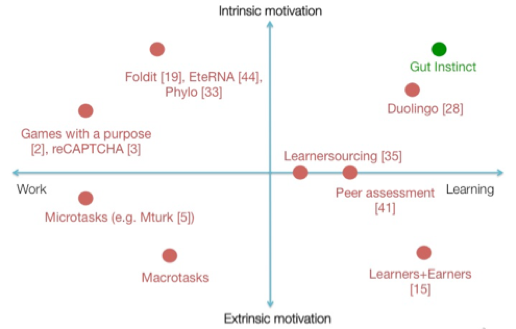
\includegraphics[width=1.0\textwidth]{figures/gutinstinct/gi-2.png}
%  \caption[]
%{Crowd systems/techniques place different emphasis on
%work and learning. Some, like Mechanical Turk~\cite{Amazon2016}, emphasize
%work over learning. Crowd approaches also vary in their motivation.
%Games like Foldit~\cite{Cooper2010} leverage participants’ motivation
%to perform altruistic work while having fun. Gut Instinct helps
%participants learn about the gut microbiome while contributing
%towards the altruistic purpose of helping researchers better
%understand it.\index{gi-2}    Refs for the fig: ~\cite{Chen2016b}   }
%  \label{fig:gi-2}
%\end{figure}

\begin{wrapfigure}{r}{0.5\textwidth}
  \centering
  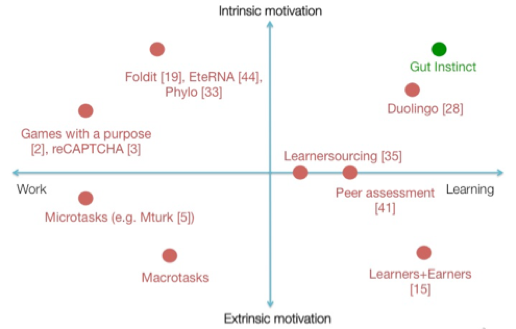
\includegraphics[width=0.5\textwidth]{figures/gutinstinct/gi-2.png}
  \caption[Crowd systems/techniques place different emphasis on
work and learning]
{Crowd systems/techniques place different emphasis on
work and learning. Some, like Mechanical Turk~\cite{Amazon2016}, emphasize
work over learning. Crowd approaches also vary in their motivation.
Games like Foldit~\cite{Cooper2010} leverage participants’ motivation
to perform altruistic work while having fun. Gut Instinct helps
participants learn about the gut microbiome while contributing
towards the altruistic purpose of helping researchers better
understand it.\index{gi-2}    \textbf{Refs for the fig: ~\cite{Chen2016b}}}
  \label{fig:gi-2}
\end{wrapfigure}

\subsection{Leveraging Crowdsourcing Successes}
Collectively aggregating many people’s responses can produce faster, better, and more reliable results---at much larger scale---than lone individuals can, at least when errors and biases are independent events~\ref{surowiecki2005wisdom}. Canonical crowdsourcing tasks have clear right or wrong answers – like whether two images represent the same product, whether an image region contains a feature, or what street number is written on a sign.

Distributing labor redundantly across multiple workers also guards against individual shortcomings~\cite{Snow2008}. For example, workers using the Soylent crowd-powered document editor found a typo late in a paper that eluded all eight authors and six reviewers~\cite{Bernstein2010a}. Why? In later pages, fatigue can reduce attention to detail. Because individual crowd workers saw only a small piece of the document, their collective attention to detail remained constant throughout. This illustrates how a collection of novices offers complementary contributions to experts, often in small but nonetheless useful ways. 

%Sometimes, having a different background than experts can be beneficial. Shared knowledge is great when it’s right, but blocks progress when wrong. When false assumptions limit experts, at least some novices are likely to be “uninfected”. For example, GalaxyZoo volunteers discovered ‘green pea’ galaxies overlooked by scientists who mistakenly assumed the green hue was merely an imaging artifact~\cite{Tinati2015}. The converse also holds, and much more often: novices are also “uninfected” by all the knowledge that enables experts to innovate. In a large distributed community, there’s often someone who happens to have important relevant knowledge, usually drawing on a relevant but distant domain. Such distributed efforts are a type of lead-user innovation~\cite{VonHippel2005a}. Having many people work on the same problem increases the odds that one will break through. Drawing on secondary expertise as inspiration can be an important agent of creativity because almost by definition, the combination is rare~\cite{Boden2004}. Open \& crowd innovation builds up on contributions by diverse online participants, and a ‘bubbling up’ process for strong ideas~\cite{Yu2012}. Our novel contribution is an explicit integration of learning.

%Crowd workers perform better when they understand their efforts’ importance. For example, Mechanical Turk workers analyzing radiology images performed better when told of the medical purpose: finding cancerous tumors~\cite{Chandler2013}. Motivation can also be personal. For example, 23andMe is a genetic testing site and online service that includes a discussion board. On this forum, a user reported disliking the sounds of others eating. She’s not alone; a 23andMe survey found 16,000 users with the same condition and a predictive genetic similarity among them~\cite{23andMe2016}.

%Creative, open-ended work has rich pedagogical value. Online work, like online learning, requires appropriate scaffoldings, such as rubrics~\cite{Boud1995, Kulkarni2013peer}, decision trees~\cite{Lee2016,Yu2006}, tutorials~\cite{Andersen2012}, and quick expert guidance~\cite{dow2012shepherding}. Similar to general critique of pure discovery learning~\cite{Mayer2004}, simply asking participants to “figure it out” would be poor pedagogy. Hence, Gut Instinct introduces a guided discovery learning approach as Mayer advocates: expert-curated learning materials help participants start, with discovery following. Recruiting learners as citizen scientists offers a Problem-based learning experience with context and motivation for the material students learn~\cite{Savery1995}. In principle, these real-world problems also provide a yardstick for measuring learning. 

%%%%%%%%%%%%%%%%%%%%%%%%%%%%
\subsection{Dual objective functions in learning and crowdsourcing}
Combining university classes in psychology with editing
Wikipedia articles led to improvement in the scientific
content of over 800 Wikipedia articles while students
learned about the topic they edited~\cite{Farzan2013}. Similarly, Kim et
al. asked learners to create how-to video segments as part
of an online curriculum~\cite{Kim2015f}; the student-created videos
then became a learning resource for the next cohort. 

Some crowdsourcing offers a dual objective: user-facing
goals include fun (e.g., Peekaboom~\cite{VonAhn2006}), authentication
(reCAPTCHA~\cite{Ahn2008}), and learning (Duolingo~\cite{Hacker2014}). Under the
hood, these tasks simultaneously label images, transcribe
text, and translate phrases. Such crowd work can also bootstrap machine learning~\cite{Bernstein2012c}. This paper is distinct from prior
work (Figure~\ref{fig:gi_2}) in leveraging people’s individual lived
experience, knowledge, context, and folk theories, rather
than treating people as interchangeable respondents.

%%%%%%%%%%%%%%%%%%%%%%%%%%%%%%%%
\section{Hypotheses}
This chapter investigates an approach for a community of learners to collaboratively create scientific theories. Learning is any endeavor that seeks to increase a participant’s knowledge. In this submission---like many MOOCs---watching videos is the main form of learning, \& quizzes are the main assessment. Work is any endeavour where the outcome has value. In this submission, authoring \& answering questions are the main work forms. This study operationalized engagement as time spent. We hypothesized that doing useful work on real-world problems helps learning, and vice versa. Specifically:

\textbf{H1. Learning improves quality of work on relevant problems.}
While learning almost by definition improves performance on similar tasks, transfer to novel tasks (like creating new \& different questions) is famously uneven~\cite{Boden2004}---and sometimes detrimental. H1 tests whether learning would improve work (e.g., novel question creation) because it marries lived knowledge (about diet, health, etc.) with a conceptual framework about the gut’s role.

\textbf{H2. Working on relevant real-world problems improves learning.}
H2 tests whether working improves learning because it increases motivation \& provides an immediately relevant ‘host context’ for new knowledge.
 
\textbf{H3. Working while learning improves learners’ engagement with the learning material.} 
For similar reasons, we hypothesized that working alongside learning would increase engagement because the two endeavors both ‘get the wheels turning’ in hopefully com-plementary ways.

We test these hypotheses in the context of brainstorming potential causal relationships in the human gut microbiome. 

%%%%%%%%%%%%%%%%%%%%%%%%%%%%%%%%%%%%
\section{The Gut Instinct System}
Gut Instinct is a collaborative system with a dual objective: help people learn about the gut microbiome, and catalyze the creation of a list of factors that may be associated with gut microbiome differences (Figure~\ref{fig:gi_3}). People anonymously post questions about lifestyle and health for peers to answer. Learners both ask \& answer questions, there are
no distinct workers. These questions and discussions provide researchers cues to build associations between lifestyle and the microbiome.
Gut Instinct is a web application built with Meteor (http://www.meteor.com). The front-end uses Angular (http://www.angularjs.org) and is stylized with Materialize (http://www.materialize.css).

\begin{figure}[h] 
  \centering
  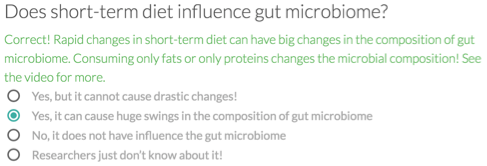
\includegraphics[width=1.0\textwidth]{figures/gutinstinct/gi-3.png}
  \caption[Gut Instinct is a web system to learn about the gut microbiome and create causal theories about gut microbiome]
{ Gut Instinct is a web system to learn about the gut microbiome and create causal theories about gut microbiome (a) A discussion board where learners add their questions and discuss them with other learners (b) "Add question" box for people to add their own questions, (c) A tutorial video showing how gut microbiome varies across countries with different food habits~\cite{Yatsunenko2012}\index{gi-3}}
  \label{fig:gi-3}
\end{figure}

\subsection{Curating content based on topics}
Gut Instinct provides expert-approved learning material including online lectures, science articles and research papers. Participants add articles they feel are useful, which can be fact-checked by experts. The gut microbiome is an active area of research with new results being generated rapidly. A popular MOOC provides an introduction to science the gut microbiome including its relation to some lifestyle choices~\cite{Knight2016}. Popular online articles about the microbiome are split between providing correct, useful information and clickbait articles without scientific validity.

\begin{wrapfigure}{R} {0.5\textwidth}
  \centering
  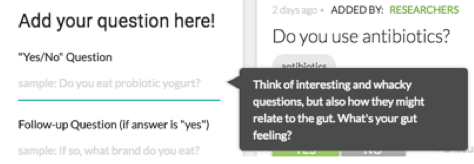
\includegraphics[width=0.5\textwidth]{figures/gutinstinct/gi-4.png}
  \caption[A question on Topics page for diet to test understanding of the learning material]
{A question on Topics page for diet to test understanding of the learning material \index{gi-4}}
  \label{fig:gi-4}
\end{wrapfigure}

Gut Instinct organizes the learning material based on topics such as diet or antibiotics. A topic-based classification of learning material provides two advantages: (a) People can deeply focus on the topics that interest them, and (b) Topics related to specific lifestyle aspects can trigger specific questions. The topics pages include videos and articles about diet, antibiotics, probiotics, physiology, and genetics based on vetted content from online sources. Quick multiple-choice questions with detailed feedback at every topic page help people test their understanding (Figure~\ref{fig:gi-4}). Overall, these elements of the interface form the learning part of the system. 

%\begin{figure}[h] 
%  \centering
%  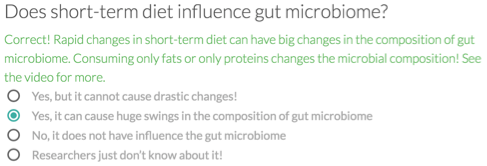
\includegraphics[width=1.0\textwidth]{figures/gutinstinct/gi-3.png}
%  \caption[]
%{A question on Topics page for diet to test understanding of the learning material \index{gi-3}}
%  \label{fig:gi-3}
%\end{figure}

%\begin{figure}[h] 
%  \centering
%  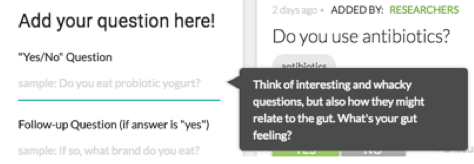
\includegraphics[width=1.0\textwidth]{figures/gutinstinct/gi-4.png}
%  \caption[]
%{An example of a nudge used in Gut Instinct to remind people of their role as a citizen scientist in raising interesting questions about the gut microbiome \index{gi-4}}
%  \label{fig:gi-4}
%\end{figure}

%\begin{wrapfigure}{R} {0.5\textwidth}
%  \centering
%  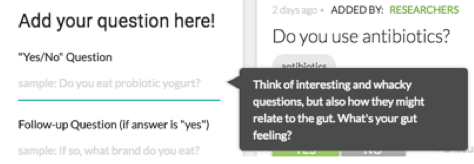
\includegraphics[width=0.5\textwidth]{figures/gutinstinct/gi-5.png}
%  \caption[Gut Instinct is a web system to learn about the gut microbiome and create causal theories about gut microbiome]
%{ Gut Instinct is a web system to learn about the gut microbiome and create causal theories about gut microbiome (a) A discussion board where learners add their questions and discuss them with other learners (b) "Add question" box for people to add their own questions, (c) A tutorial video showing how gut microbiome varies across countries with different food habits~\cite{Yatsunenko2012} \index{gi-5}}
%  \label{fig:gi-5}
%\end{wrapfigure}

%\begin{wrapfigure}{R} {0.5\textwidth}
%  \centering
%  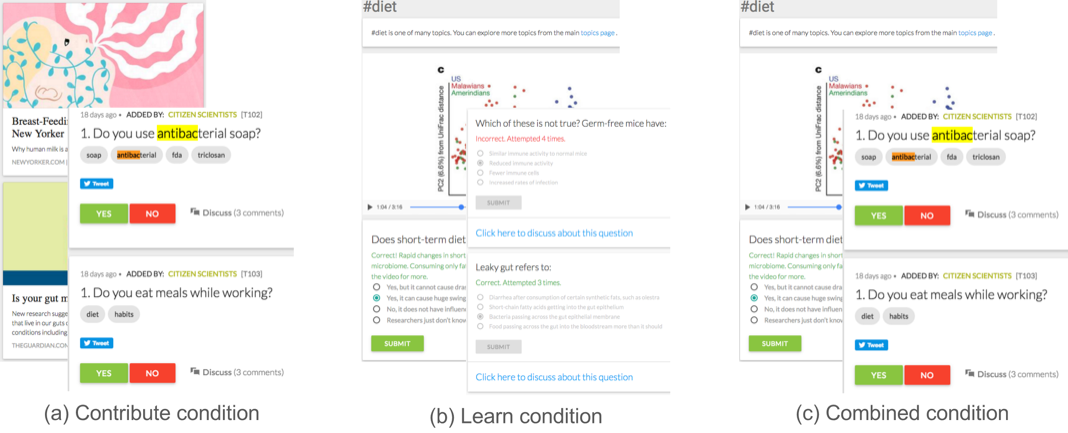
\includegraphics[width=0.5\textwidth]{figures/gutinstinct/gi-6.png}
%  \caption[Three conditions for experiment]
%{Three conditions for experiment. (a) Contribute condition where participants read some general articles about microbiome and added questions and answered others’ questions (b) Learn condition where participants saw curated topic videos (e.g. about diet) and answered practice problems from a Coursera class~\cite{Knight2016} (c) Combined condition where participants saw curated topic video, and added questions and answered others’ questions \index{gi-6}}
%  \label{fig:gi_6}
%\end{wrapfigure}

\subsection{GutBoard: Discussing and answering questions}
The GutBoard provides a discussion board with user-generated questions tagged by topics (Figure~\ref{fig:gi_3}(a)). People can browse questions, answer them, or participate in discussions. GutBoard presents unanswered questions first. The most popular questions (in terms of discussion comments) bubble to the top of the board.
 
\subsection{Adding questions}
Gut Instinct provides different tutorials, articles, and expert examples to help users contribute. Gut Instinct requires that questions have a two-part structure: a yes/no question followed by an open-ended elaboration. For example, the yes/no question “Do you take any meal replacements such as protein powders?” might be followed by “Do you take them on a daily basis?” This structure addresses two problems we witnessed with pilot users: (a) Some questions were actually multiple different questions, confusing readers (b) Readers had to read every question in full to understand what was being asked, even if the topic was not relevant to them. With this structure, every question has a single focused topic. Participants can also start a discussion about the question and provide relevant tags. “Add Question” box in Figure~\ref{fig:gi_3}(b) shows the interface.

\subsubsection{Nudges to think creatively and to stay on task}
Gut Instinct employs several best practices for increasing high-quality contributions~\cite{Jennett2014, Resnick2011}. It provides cues to teach participants to generate good questions. All parts of the Add Question box contained sample questions to help participants frame their questions that could be useful to them and to gut microbiome researchers (Figure~\ref{fig:gi_5}). To reduce user confusion, GutBoard was seeded with expert questions that set norms for the nature of questions. To provide a clear call to action, GutBoard was the default landing page and the only place to add or view questions. Every page had a tour that users could invoke anytime to learn its interface.

%todo-uncomment -- don't know what's wrong
\begin{wrapfigure}{b} {0.5\textwidth}
  \centering
  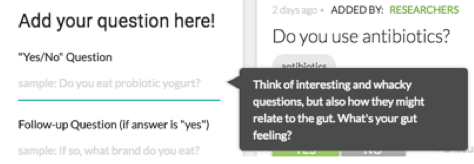
\includegraphics[width=0.5\textwidth]{figures/gutinstinct/gi-5.png}
  \caption[An example of a nudge used in Gut Instinct]
{An example of a nudge used in Gut Instinct to remind people of their role as a citizen scientist in raising interesting questions about the gut microbiome \index{gi-5}}
  \label{fig:gi-5}
\end{wrapfigure} 

%%%%%%%%%%%%%%%%%%%%%%%%%%%%%%%%%%%%%%%%
\section{Experiment: Work, Learning, \& Combined}
A between-subjects experiment compared the work and learning performance of participants across three different conditions: \textit{Contribute}, \textit{Learn} and \textit{Combined} (Figure~\ref{fig:gi_6}). In the Learn condition, participants were provided learning material and some practice problems, both curated from the Coursera microbiome class~\cite{Knight2016}). In the Contribute condition, they had access to brief pop-science articles to know basic details about the gut microbiome, and GutBoard for creating questions. In the Combined condition, subjects had access to both learning material from Coursera and the GutBoard. The GutBoard content was common to both conditions that used it (Contribute and Combined).

\begin{figure}[h]
  \centering
  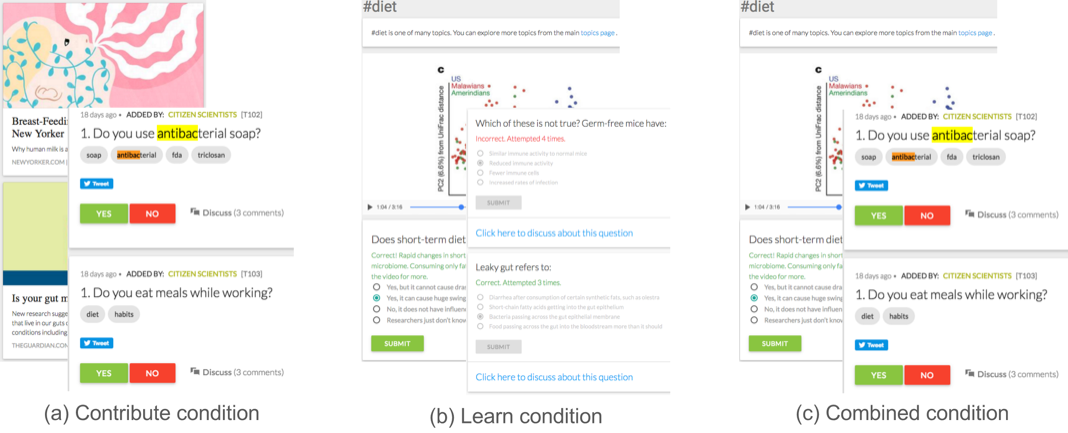
\includegraphics[width=1.0\textwidth]{figures/gutinstinct/gi-6.png}
  \caption[Three conditions for experiment]
{Three conditions for experiment. (a) Contribute condition where participants read some general articles about microbiome and added questions and answered others’ questions (b) Learn condition where participants saw curated topic videos (e.g. about diet) and answered practice problems from a Coursera class~\cite{Knight2016} (c) Combined condition where participants saw curated topic video, and added questions and answered others’ questions \index{gi-6}}
  \label{fig:gi_6}
\end{figure}

\subsection{Method}
Participants were randomly assigned to one of the three conditions. Each comprised an individual lab session followed by web study, during which participants were asked to use the tool for 3 days. During this period, participants asked and answered each others’ questions in the tool.

\textit{Lab}: A researcher introduced the condition-appropriate Gut Instinct site. Participants were told there was no lower or upper limit on how much time to spend using the system. Each session comprised the following steps: (1) accessing the consent form, (2) seeing GutBoard/problems, (3) accessing topic videos/articles, and (4) participating in a short interview. The interview asked participants about their knowledge of the gut microbiome before using the system, and their experience using the system. The interview was tailored to the participant’s behavior: for example, if a participant did not click on Google Scholar references inside Gut Instinct but opened up a browser for web search, the interviewer would ask why.
 
\textit{Web usage}: Once all participants had completed the lab portion, the web application was opened to all participants for collaborative usage for three days. Gut Instinct sent email notifications about activity on the site, along with feedback on some questions raised on GutBoard such as providing links to research studies about effects of eating blueberries on the gut microbiome. 

After web usage, two independent raters (experts in human microbiome) rated the questions on novelty \& usefulness using the following workflow: (1) calibrate: rate 3 questions independently and discuss; (2) rate: independently rate all participant generated questions; (3) combine: discuss ratings where different \& develop a common score. The discussion in step 3 was valuable for adding to the set of rules for rating such open-ended questions. 

%%%% TABLE 2 %%%%
\vspace{0.25in}
\begin{table}[!ht]
\caption[Demography info for 44 participants. Some participants did not complete portions of survey]{Demography info for 44 participants. Some participants did not complete portions of survey}

\vspace{-0.25in}
\begin{center}
%\setlength{\tabcolsep}{10pt} % Default value: 6pt
\renewcommand{\arraystretch}{1.5} % Default value: 1
%\begin{tabular}{c >{\em}c c}
\begin{tabular}{|>{\bf}p{1.5in}|p{1.5in}|p{1.5in}|}
\hline
Nationality	&	Indian = 22	&	Non-Indian = 22\\
Gender		&	Female = 7	&	Male = 37\\
Age			&	18-20 = 1		& 	26-30 = 19\\
			&	21-26 = 14	&	31-35 = 5\\
Ethnicity		&	Indian = 18	& 	Caucasian= 11\\
			&	Asian/Pacific Islander= 5	&	Hispanic/Latino = 2\\
			&	Others/Not said = 4	 &				\\
Current		& 	Undergraduate = 3	& Ph.D. = 29\\
 educational status 	&	Masters = 7	&	Postdoc = 2\\
\hline
\end{tabular}
\end{center}
\label{tab:gi-demo}
\end{table}

\subsection{Participants}
44 participants were recruited from a Southern California university (Table~\ref{tab:gi-demo}). Participants were novices in terms of their knowledge of the human microbiome. Random assignment balanced g ender and nationality across conditions. There were equal numbers of women---and equal numbers of men---in each condition. Where not evenly divisible by 3, one condition had one more or fewer. 


\subsection{Measures}
Dependent variables comprised work (number of questions contributed, novelty and usefulness measured by blind, independent raters); learning (score on summative test); and engagement (time spent during lab session, and number of discussion comments during web usage). Qualitative measures included how participants used the tool, where they got stuck, how they collected info, which questions they engaged with, and a post-experiment survey.

\subsection{Results}
Analysis of variance estimated the effect of working, learning and the work-learn interaction. Two condition comparisons used a Mann-Whitney U test with the corresponding independent variable (learning or working). 

\begin{figure}[h] 
  \centering
  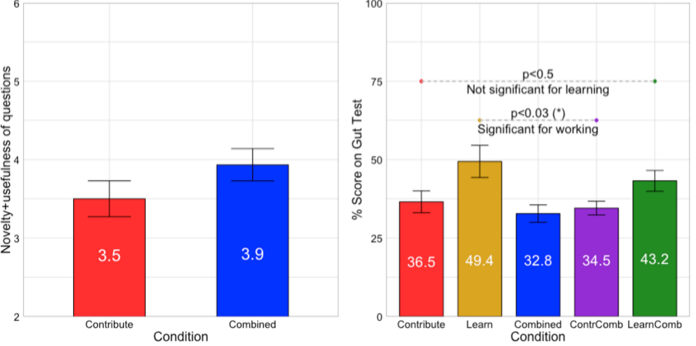
\includegraphics[width=1.0\textwidth]{figures/gutinstinct/gi-7.png}
  \caption[Results: Question quality, Learning Score, and Time Spent]
{a) Participants in Contribute and Combined conditions created questions of similar quality b) Participants in Learn condition performed the best on a summative test. Learning did not show a significant effect on score but working did c) There were no significant differences in time spent in lab session across the conditions \index{gi-7}}
  \label{fig:gi-7}
\end{figure}

\textit{Work}: Did access to Coursera learning material (Combined) impact quantity and quality of questions relative to not having access (Contribute)? The Combined participants generated questions of similar novelty and usefulness (M = 3.5) as Contribute participants (M = 3.93), Mann–Whitney U = 79, n1 = 14, n2 = 15, p < 0.23 two-tailed (Figure~\ref{fig:gi_7}a). Figure~\ref{fig:gi_8} shows two examples of questions rated by experts. Ten of the 29 questions mirrored questions found on the American Gut survey. Half of the participants’ questions (14 of 29) asked about diet. Participants in Combined and Contribute conditions generated a total of 14 and 15 questions, respectively, averaging one question per participant (see Figure~\ref{fig:gi_9}). 

\textit{Learning}: Did participants instructed to ask questions (Contribute \& Combined) score differently than those who were not (Learning)? Did access to learning videos (Learning \& Combined conditions) impact quiz scores relative to not having access (Contribute)? A two-factor ANOVA estimated these effects, finding significantly lower scores for those requested to ask questions. By contrast, access to learning materials did not yield a significant difference in quiz score.

The Learn participants performed scored higher (M = 5.93) on Learning test than participants in Combined (M = 4.38) or Contribute (M = 3.93) conditions. An analysis of variance showed that this effect was significant for working, F(1, 39) = 5.22, p < 0.03, but not for learning, F(1, 39) = 0.46, p < 0.5 (Figure~\ref{fig:gi_7}b). The effect size for working was small (Cohen’s effect size d = .11).

Engagement: The mean length of lab session was ~20 min (varying from 9-40 min). Learn participants spent marginally more time (M = 26.9 min) in the lab session than participants in Combined (M = 22.5 min) or Contribute (M = 16.7 min) conditions. An analysis of variance showed that this effect wasn’t significant for either Learning F(1, 41) = 3.40, p < 0.07 or working F(1, 41) = 1.95, p < 0.17, (Figure~\ref{fig:gi_7}c). Combined and Contribute participants contributed 35 discussion comments each; Learn participants contributed 10 discussion comments.

38 of 40 correspondents reported prior use of online courses, varying from occasional use of online learning material to taking more than five online classes. Preliminary analyses found no effects for gender and nationality (Indian or non-Indian), so these were excluded from further analyses. Table~\ref{tab:gi-results1} summarizes results from the experiment. 

%%%% TABLE 2 %%%%
\vspace{0.25in}
\begin{table}[!ht]
\caption[Summary of results from experiment]{Summary of results from experiment}

\vspace{-0.25in}
\begin{center}
%\setlength{\tabcolsep}{10pt} % Default value: 6pt
\renewcommand{\arraystretch}{1.5} % Default value: 1
\begin{tabular}{|p{1in}|p{1in}|p{1in}|p{1in}|p{1in}|}
\hline
Measures(mean values)	& Combined &	Contribute	& Learn	& {\it p} \\
\multicolumn{5}{|l|}{\bf No difference in quality or quantity of questions across Combined or Contribute conditions}   \\
Quality of questions (2-6 scale)  &	3.5 &	3.93	&-	& $<$ .23\\
\# of questions/\# of participants &	14/14 &	15/15 &	- &	-\\
\multicolumn{2}{|l|}{\bf  Working reduced test scores}  & & & \\
Test score (max: 12 points) & 4.38	& 3.93 & 5.92 & L $<$ .5, W $<$ .03 \\
\multicolumn{5}{|l|}{\bf Learning or contributing did not have a significant effect on time spent in lab }   \\
Time taken in lab session (min) & 22.5 & 16.7 & 26.8 & L $<$ .07, W $<$ .17\\
\# of discussion comments & 35 & 35 & 10 & - \\
\hline
\end{tabular}
\end{center}
\label{tab:gi-results1}
\end{table}

\begin{figure}[h] 
  \centering
  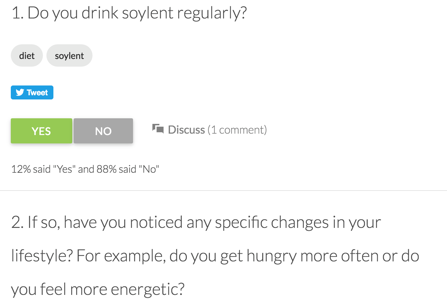
\includegraphics[width=0.48\textwidth]{figures/gutinstinct/gi-8a.png}
  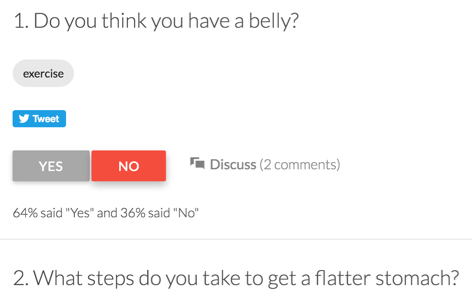
\includegraphics[width=0.48\textwidth]{figures/gutinstinct/gi-8b.png}
  \caption[Examples of questions added by participants]
{An example of a good and bad question added by participants. Soylent question was scored 5/6 (2 on novelty and 3 on usefulness) while the belly question was rated 2/6 (1 on novelty and 1 on usefulness) \index{gi-8}}
  \label{fig:gi-8}
\end{figure}


\begin{figure}[h] 
  \centering
  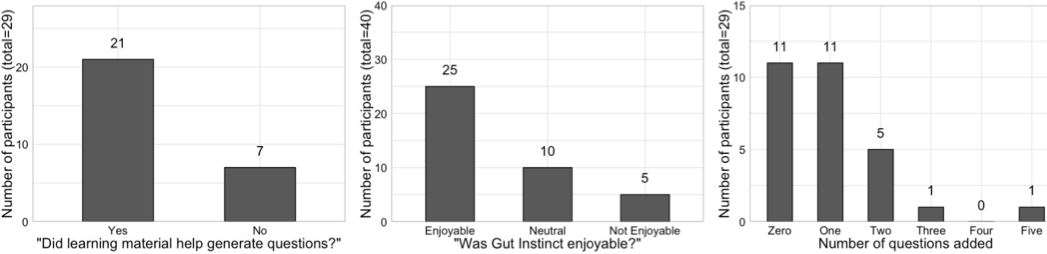
\includegraphics[width=1.0\textwidth]{figures/gutinstinct/gi-9.png}
  \caption[Participants' self-reports]
{Most participants reported that the learning experience was helpful and the system was enjoyable. 65\% of participants asked questions; the mode was 1) \index{gi-9}}
  \label{fig:gi-9}
\end{figure}

%%%%%%%%%%%%%%%%%%%%%%%%%%%%%%%%%
\section{Discussion}
These results suggest that some learners create useful research questions based on their lifestyle but its effect on better learning is unclear.

\textit{Why did Learn participants perform better on tests?}
Learn participants had a clear objective: learn about the gut microbiome, practice problems related to it, and take a summative test. By contrast, participants in the other two conditions had to both generate novel questions and take the summative test. They may have placed less emphasis on the test. Generating questions and taking test on a novel topic might have required greater effort than what the participants wanted to put in. Additionally, difficulty of creating questions may have lowered participants’ confidence in taking the test. 

\textit{Personalized learning and need for feedback}
Participants were curious to know the microbiome science behind disclosed aspects of their lifestyle. One participant commented, “After answering the question, I would expect to see some succinct information about where my lifestyle stands with respect to scientific wisdom.” Participants also asked for a section curated for them by the tool, or a section where they could save items of personal relevance.
 
\textit{Need for self-directed learning}
Online learning material provided useful information about a complex topic like the microbiome hoping that it might spur participants to find and use other similarly trustworthy sources of their liking. In the lab, participants used web search to find relevant resources. Most participants reported that they did not search at home. 

\textit{Learning did not improve quality of work}
Combined participants did not generate questions of higher quality than those without learning material (Contribute condition). Crowdclass~\cite{Lee2016} found similar results where workers who simply classified images did better than those who learned about decision trees and subsequently classified images as an assignment. How do online learning materials and useful work tie to each other? Gut Instinct explored one design point where learning and working were provided specific components in the tool to reduce participant confusion. An alternate approach could be to have a work-biased design where learning material would be tailored to participants’ questions or a learn-biased design where participants could add questions only in the specific context of learning materials. For instance, people could raise questions at different point of a topic video~\cite{Lee2015b} rather than using a separate part of the tool.
 
\textit{Difficulty of generating questions}
A remarkable and concrete measure of participants’ insights is that ten of their questions mirrored those asked by the American Gut survey~\cite{KnightLab2016}. Unsurprisingly, other participants reported difficulty creating good questions. Asking questions is a valuable metacognitive experience that can be scaffolded by examples of good questions from experts. 

Gut Instinct sent email asking people to contribute, reminding them of the importance of their task, and showing successful examples of citizen science work. Such reminders 
prompted a temporary increase in questions increased or discussion contributions~\cite{Kotturi2015} but did not lead to a sustained stream of questions and discussions. Some participants complied with the letter of the request but not the spirit by taking a sample question and tweaking it slightly.

\textit{What kind of innovation can we expect from citizen science}
Half of participants’ questions were about diet. Diet offers both a clear influence mechanism and immediate personal relevance. While a compelling video about effect of diet on the microbiome likely helped, a video alone appears insufficient: for instance, the topic of genetics also had a video, but no participants asked questions about genetics. Moreover, many diet questions are perceived as less personally disclosive than genetics questions.
 
That participants asked many questions about diet and none about genetics is consistent with patterns of where lead users innovate, and where they don’t~\cite{VonHippel2005a}. Lead-user innovation works best for “need-intensive” problems where people’s lived experiences provide the key ingredient, e.g., a snowboarder who cuts their boots to improve fit. These innovations arise through trial and error, and solution efficacy is readily observable. Lead-user innovation is less common with “solution intensive” problems, where highly technical knowledge, access to equipment, and/or significant financial capital are critical. 
 
\textit{Does browsing displace contributing?}
Participants spent most of the lab session browsing discussions and learning material. By our observation, later participants spent more time using the system in the lab. Despite spending more time browsing discussions, we think later participants added fewer questions. Participants mentioned that browsing and answering questions felt like “contributing” without putting in a lot of effort. Participants also reported that they had to break a mental barrier to publicly post a discussion comment or question. 

\subsection{Limitations}
Participants could login as little or as many times as they wished. One participant commented that even though she had some ideas to add, she was conscious of disclosing information about her personal life (participants were anonymous). It may be that using the tool in an experiment made them more cautious of what they added or commented.
As a web application, participants assumed comparable facilities to forum/ discussion sites like Quora. This exemplifies a challenge of testing research prototypes: the absence of production-level features can change participants’ impressions and possibly their behavior.

%%%%%%%%%%%%%%%%%%%%%%%%%%%%%%%%%%%%
\section{Science with Learners: Promise \& Challenges}
This chapter investigated the merits of combining learning and contributing. While experimental results did not show the hypothesized additive benefits, we still believe this combination has potential. Is it intrinsically self-contradictory to ask learners to contribute scientific ideas? Not necessarily. In addition to the diversity benefits that the global community brings, those with brand new knowledge can, for example, give useful feedback to peers~\cite{Kulkarni2013peer}. Furthermore, the newly-aware sometimes articulate useful insights that familiarity has blinded experts to~\cite{Hinds1999}. Drawing on the results, related literature, and our intuitions, here are avenues that might find additive benefits where this experiment did not.

\textit{Aligning objectives}
The chapter’s experiment gave participants two objectives: take a summative test and generate ideas for lifestyle-microbiome relationships. While both relate to the same general topic---the microbiome---the “doing” of each was quite different. For example, the question that the fewest participants answered correctly asked which type of bacteria population would be affected by a behavior change. While the test emphasized specific biological facts like this, participants’ GutBoard questions were much more general. Consequently, it is not surprising that success on one didn’t catalyze success on the other. Conversely, given the mild negative correlation, it seems likely that time spent on one might have taken away from time spent on the other. More tightly aligning the test of learning with the work activities could yield the additive benefits we seek. (We say “test of learning” because participants may indeed have learned more in ways not measured.) 

We also hypothesize that an additive benefit is more likely when the knowledge and/or motivation generated by one activity transfers to the other. While this may seem obvious in retrospect, the loose-connection problem observed here may be relatively common. We hope the results warn against this risk.

\textit{Make learning \& work personally relevant}
Many American Gut Project (AGP) participants exhibit a strong intrinsic motivation to learn more about why they have a particular microbiome~\cite{Debelius2016}. The students who participated in this experiment may not have equivalently strong motivation. Motivated users may increase the quality of citizen science work. For instance, AGP participants could organize a focused effort around a specific health issue like Type 1 diabetes or Inflammatory Bowel Disease (IBD). Similar to how Wikipedia editors co-ordinate efforts~\cite{Krieger2009} using Gut Instinct with more differentiated roles like question generation, question ranking, and literature search might lead to further distinguishing work.

\textit{Learning \& working: integrate \& provide clear criteria}
We believe that integrating learning and work will be mutually beneficial when learning new material immediately opens up the possibility of contributing useful work and contribution solicitations include relevant learning material. This extends problem-based learning~\cite{Savery1995} and just in time learning~\cite{Bolton1999} to the scale of Internet. For example, browsing StackOverflow before fixing programming questions leads to better work, and lateral learning~\cite{Mamykina2011}. Similarly, global-scale distributed contributions like peer review have enabled massive online courses to offer creative, open-ended assignments through peer review~\cite{Kulkarni2013peer}. Such active learning approaches seek a dual objective of content learning and metacognitive growth~\cite{Crouch2001}.
 
Reflection and curiosity play a similar orienting role: having people guess the answer to a task-relevant question before performing the main task led to better performance on the task when hints were revealed to maintain the curiosity of the learners~\cite{Aleven2006, Law2016a}. Similarly, the surprise that arises from making a guess that’s revealed to be wrong generates a “teachable moment” for learners. How might we use these lessons for online learners to teach themselves about specific domains while performing useful work? 

\textit{Other fields for this approach}
Many other fields may benefit from the diverse contexts that online citizen scientists offer. For example, 96\% of psychology experiments used participants from Western industrialized countries~\cite{Henrich2010a}. Recent attempts have started to collect and analyze data about people all across the world by offering them fun-based rewards in lieu of collecting data about their online interactions~\cite{Reinecke2015}. Success of such initiatives hints at a motivated set of online participants who could also benefit from learning about cultural psychology concepts in more depth while undertaking relevant scientific work. 

\textbf{Conclusion}
This chapter investigated techniques for integrating learning and citizen science for the benefit of both. For us, the most striking result is that users contributed many causal questions of sufficient novelty and importance that they only recently have emerged in the literature. It is possible that other of the causal questions will be borne out in the future. This study also illustrates the challenges of double-bottom-line work. Specifically, these dual objectives can be in tension rather than being additive. The chapter describes the Gut Instinct system and suggests strategies that may help the dual objectives enhance each other. Looking forward, we hope the approach introduced here will find value in other domains especially where the science is nascent and/or contextual information is key. The knowledge of science impacts a diverse planet; in the future, this diverse community may importantly contribute to it.




